\section{Administrative Area}
The Administrative processes are performed by the gorup of employee grouped in the Admnistrative Organizational unit according to the Working Structure in figure \ref{2img:wstruct}. In particular all the processes are supervised by the CEO who is the leader of the organizational's trend.


\subsection{Billing}
This process provides support for the definition of the appropriate
remuneration for the service supplied.
The process takes into account the history of project development and the details defined in the contract, in order to check if they match or if some extra features have been during the development phase. The employees mainly involved are Business Consultant, Secretary and the CEO.

Image \ref{2img:billing} shows how this process is realized in practice, focusing on the resources used and the targets for each activity. The goal of this process is to provide a fair billing to the customer, balanced on the services actually delivered.\\

\begin{figure}[ht!]
\begin{centering}
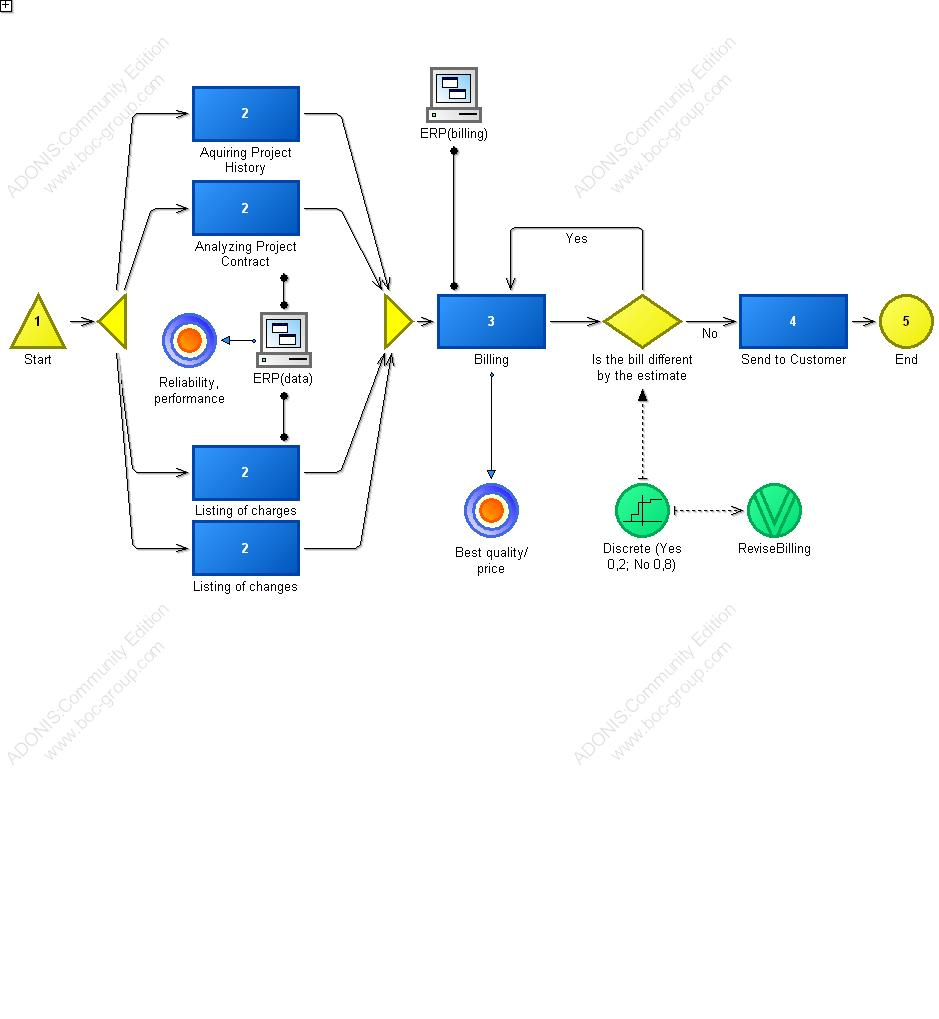
\includegraphics[scale=0.50, angle=90]{assign2/adonis/imgs/billing.jpg}
\caption{AllSpark billing process.}
\label{2img:billing}
\end{centering}
\end{figure}


\noindent
\emph{Path Analysis}\\
The analysis of possible paths results five correspondence, one with the 80,40\% of probability to be performed. For simulation's convention the number of these processes per month is configured on three element on average.

\begin{alltt}
Probability:   80,4000\%
Execution time:  00:000:00:24:20
Waiting time:  00:000:00:05:00
Resting time:  00:000:00:11:10
Transport time:  00:000:00:01:00
Cycle time:  00:000:00:29:20
Costs:  27,100000

Billing 0.3 (Business process model)

========================================
Process start: Start
Parallelity: Parallelity-25245
    *
    Activity: Aquiring Project History
    *
    Activity: Analyzing Project Contract
    *
    Activity: Listing of charges
    *
    Activity: Listing of changes
Merging: Merging-25248
Activity: Billing
Decision: Is the bill different by the estimate --> ReviseBilling = 'No'
Activity: Send to Customer
End: End
\end{alltt}

\noindent
\emph{Capacity Analysis}\\
The capacity analysis of the process illustrates the specified timing and costs forseen for the single activities. Morevover it exlicities the Performer associated to each activity in order to check the responsibility for each step of the Business Process.

\begin{table}
\centering
{\tiny
\begin{tabular}{|l|l|l|l|l|l|l|}
Business process&Activity&Performer&Number&Execution time&Cycle time&Costs\\
\hline
Billing 0.3&&&&00:000:00:24:51&00:000:00:32:42&33,575000\\
\hline
&Aquiring Project History &&1,000000&00:000:00:10:00&&1,300000\\
\hline
&&Secretary&1,000000&00:000:00:10:00&&1,300000\\
\hline
&Analyzing Project Contract &&1,000000&00:000:00:10:00&&0,200000\\
\hline
&&Secretary&1,000000&00:000:00:10:00&&0,200000\\
\hline
&Listing of charges &&1,000000&00:000:00:01:00&&0,300000\\
\hline
&&Business consultant&1,000000&00:000:00:01:00&&0,300000\\
\hline
&Billing &&1,259000&00:000:00:02:31&&31,475000\\
\hline
&&Business consultant&1,259000&00:000:00:02:31&&31,475000\\
\hline
&Listing of changes &&1,000000&00:000:00:01:00&&0,200000\\
\hline
&&Secretary&1,000000&00:000:00:01:00&&0,200000\\
\hline
&Send to Customer &&1,000000&00:000:00:00:20&&0,100000\\
\hline
&&Secretary&1,000000&00:000:00:00:20&&0,100000\\
\hline
Total&&&&00:000:00:24:51&&33,575000
\end{tabular}
}
\caption{Capacity analysis for Billing.}
\end{table}
%

%

\subsection{Bureaucracy Management}
The "Bureaucracy Management" business process aims to regulate the set of codes from which AllSpark depends on. The scope of this sequence is monitoring the country laws and the licences estabilished, check the efficiency of the responsibility charge and undertake the needed changes to restore the legality.

Since the task is actual demanding the roles it has associated are all fitting the "Administrative" organizational unit according to the Working structure in \ref{sec:working_structure}. Particular the secretary is directed the mainly connect to all of the activities as described in the above structure.

The figure \ref{2img:bureaucracy} shows the graphical representation, focusing on the management side of the topic than the pratical step.\\

\begin{figure}[ht!]
\begin{centering}
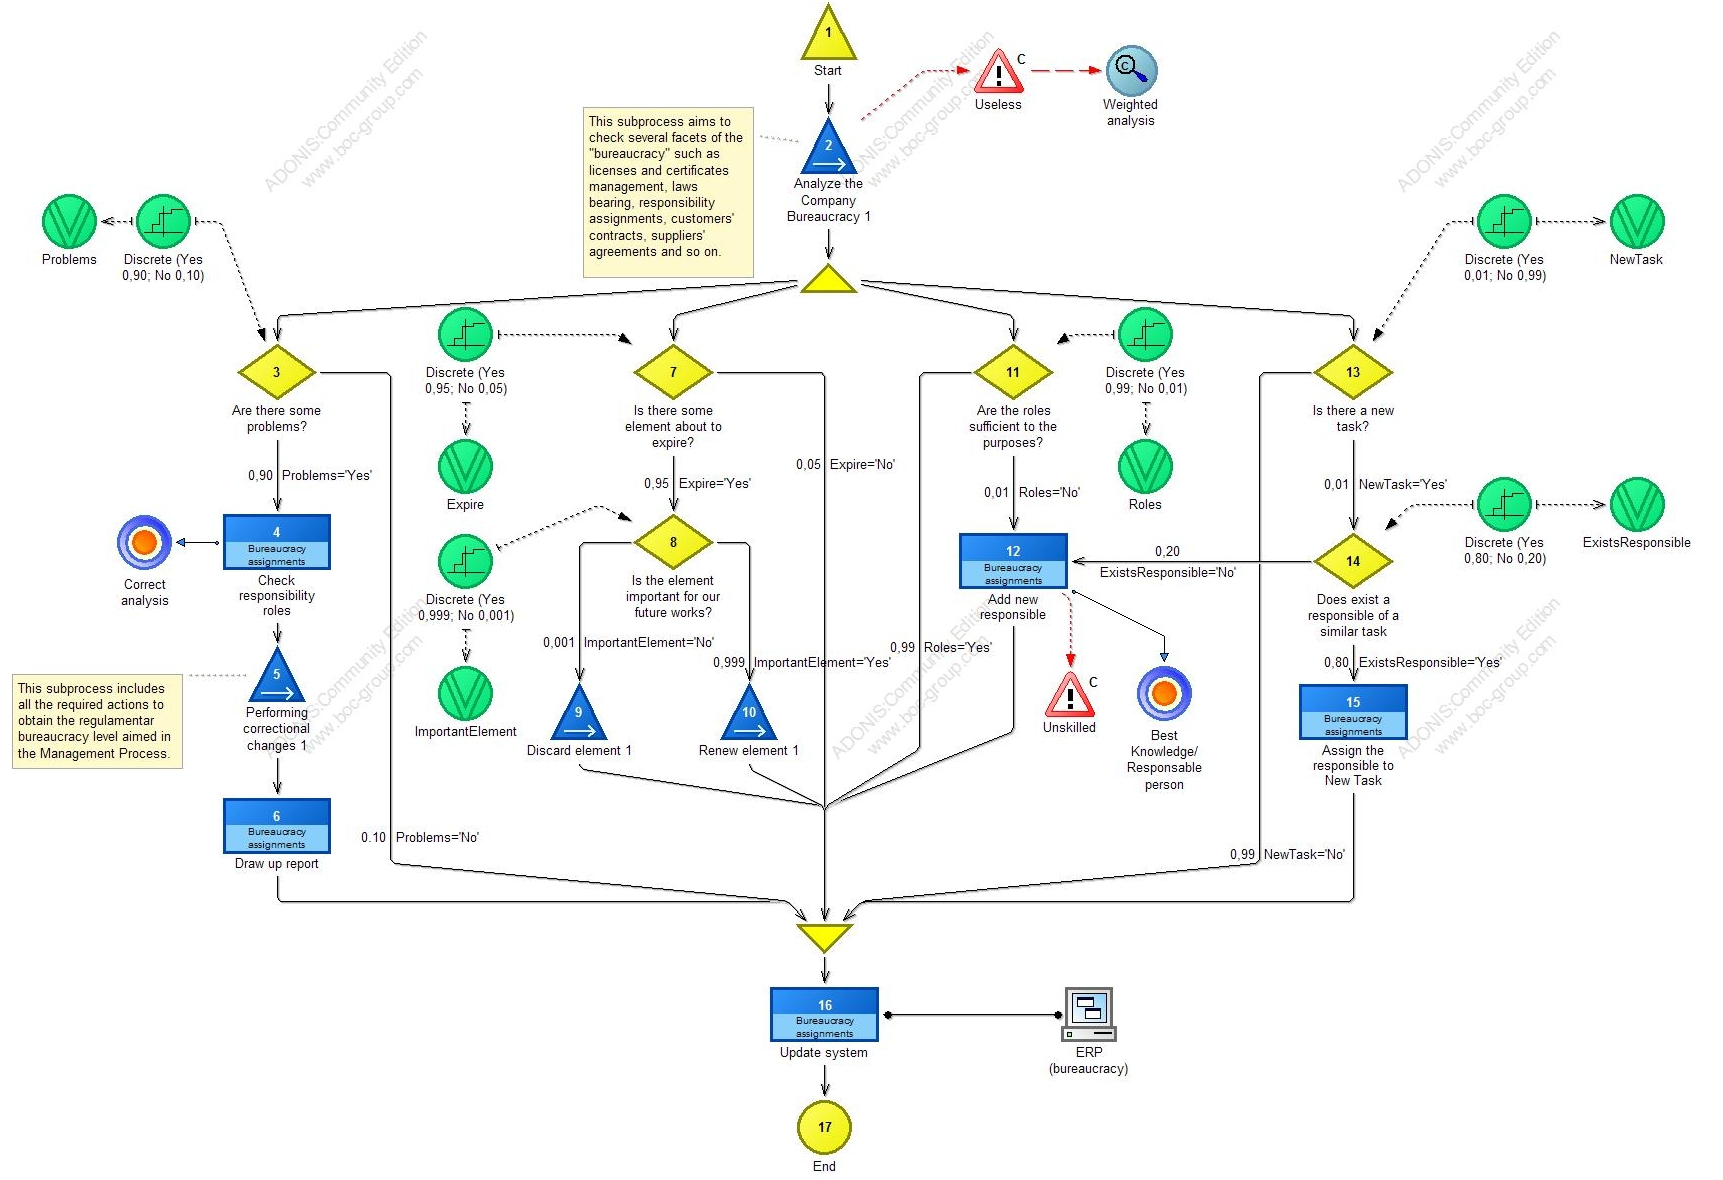
\includegraphics[scale=0.35, angle=90]{assign2/adonis/imgs/bureaucracy.jpg}
\caption{AllSpark bureaucracy management.}
\label{2img:bureacracy}
\end{centering}
\end{figure}

\noindent
\emph{Path Analysis}\\
Ten paths were discovered by the analysis of the modelization; the first leads with the 84,70\% probability to be performed. 

\begin{alltt}
Probability:   84,7000\%
Execution time:  00:000:01:55:00
Waiting time:  00:000:00:11:00
Resting time:  00:000:00:16:00
Transport time:  00:000:00:15:00
Cycle time:  00:000:01:55:00
Costs:  2030,850000

Bureaucracy Management 0.1 (Business process model)
========================================
Process start: Start
Subprocess: Analyze the Company Bureaucracy
Parallelity: Parallelity-37827
    *
    Decision: Are the roles sufficient to the purposes? --> Roles='Yes'
    *
    Decision: Is there a new task? --> NewTask='No'
    *
    Decision: Are there some problems? --> Problems='Yes'
    Activity: Check responsibility roles
    Subprocess: Performing correctional changes
    Activity: Draw up report
    *
    Decision: Is there some element about to expire? --> Expire='Yes'
    Decision: Is the element important for our future works? --> ImportantElement='Yes'
    Subprocess: Renew element
Merging: Merging-37855
Activity: Update system
End: End

Bureaucracy Management 0.1 (Business process model) --> Analyze the Company Bureaucracy 1 (Business process model)
========================================
Process start: Start
Activity: Analyze the Company Bureaucracy
End: End

Bureaucracy Management 0.1 (Business process model) --> Renew element 1 (Business process model)
========================================
Process start: Start
Activity: Renew element
End: End

Bureaucracy Management 0.1 (Business process model) --> Performing correctional changes 1 (Business process model)
========================================
Process start: Start
Activity: Performing correction
End: End
\end{alltt}

\noindent
\emph{Capacity Analysis}\\
In the capacity analysis of the process reported below, is possible to observe that the task is very wasting both in terms of time and in costs.

It is important to underline that the Process is defined to be performed at least once a month.

\begin{landscape}
\centering
{\tiny
\begin{tabular}{|l|l|l|l|l|l|l|}
Business process&Activity&Performer&Number&Execution time&Cycle time&Costs\\
\hline
Bureaucracy Management 0.2&&&&00:000:01:46:01&00:000:01:49:03&1919,760040\\
\hline
&Check responsibility roles&&0,899000&00:000:00:26:58&&26,970000\\
\hline
&&Secretary&0,899000&00:000:00:26:58&&26,970000\\
\hline
&Add new responsible&&0,010000&00:000:00:00:09&&0,000500\\
\hline
&&Secretary&0,010000&00:000:00:00:09&&0,000500\\
\hline
&Update system&&1,000000&00:000:00:05:00&&0,050000\\
\hline
&&Secretary&1,000000&00:000:00:05:00&&0,050000\\
\hline
&Draw up report&&0,899000&00:000:00:17:59&&0,179800\\
\hline
&&Secretary&0,899000&00:000:00:17:59&&0,179800\\
\hline
&Assign the responsible to New Task&&0,009000&00:000:00:00:01&&0,000090\\
\hline
&&Secretary&0,009000&00:000:00:00:01&&0,000090\\
\hline
&Analyze the Company Bureaucracy&&1,000000&00:000:00:10:00&&0,200000\\
\hline
&&Secretary&1,000000&00:000:00:10:00&&0,200000\\
\hline
&Performing correction&&0,899000&00:000:00:26:58&&0,359600\\
\hline
&&Secretary&0,899000&00:000:00:26:58&&0,359600\\
\hline
&Renew element&&0,946000&00:000:00:18:55&&1892,000000\\
\hline
&&Secretary&0,946000&00:000:00:18:55&&1892,000000\\
\hline
&Discard element&&0,001000&00:000:00:00:00&&0,000050\\
\hline
&&Secretary&0,001000&00:000:00:00:00&&0,000050\\
\hline
Total&&&&00:000:01:46:01&&1919,760040
\end{tabular}
}
%\caption{Capacity analysis for Bureaucracy Management.}
\end{landscape}
%

%

\subsection{Financial support}
The "Financial support" business process wokrs on the management of the Company's financial status with monitoring the growing opportunities as primary target, but not least also to check the AllSpark's trend in order to mantain the position gained. Reliability is a important objecttive to reach in this process since a wrong planning may have serious reflections in the future of the Company (and, of course, of its employees).

The primary responsible of all the business process is the business consultant who is assisted by the secretary and supervised for decision by the CEO.

The figure \ref{2img:financial_sup} reports the representation of the discussion.\\

\begin{figure}[ht!]
\begin{centering}
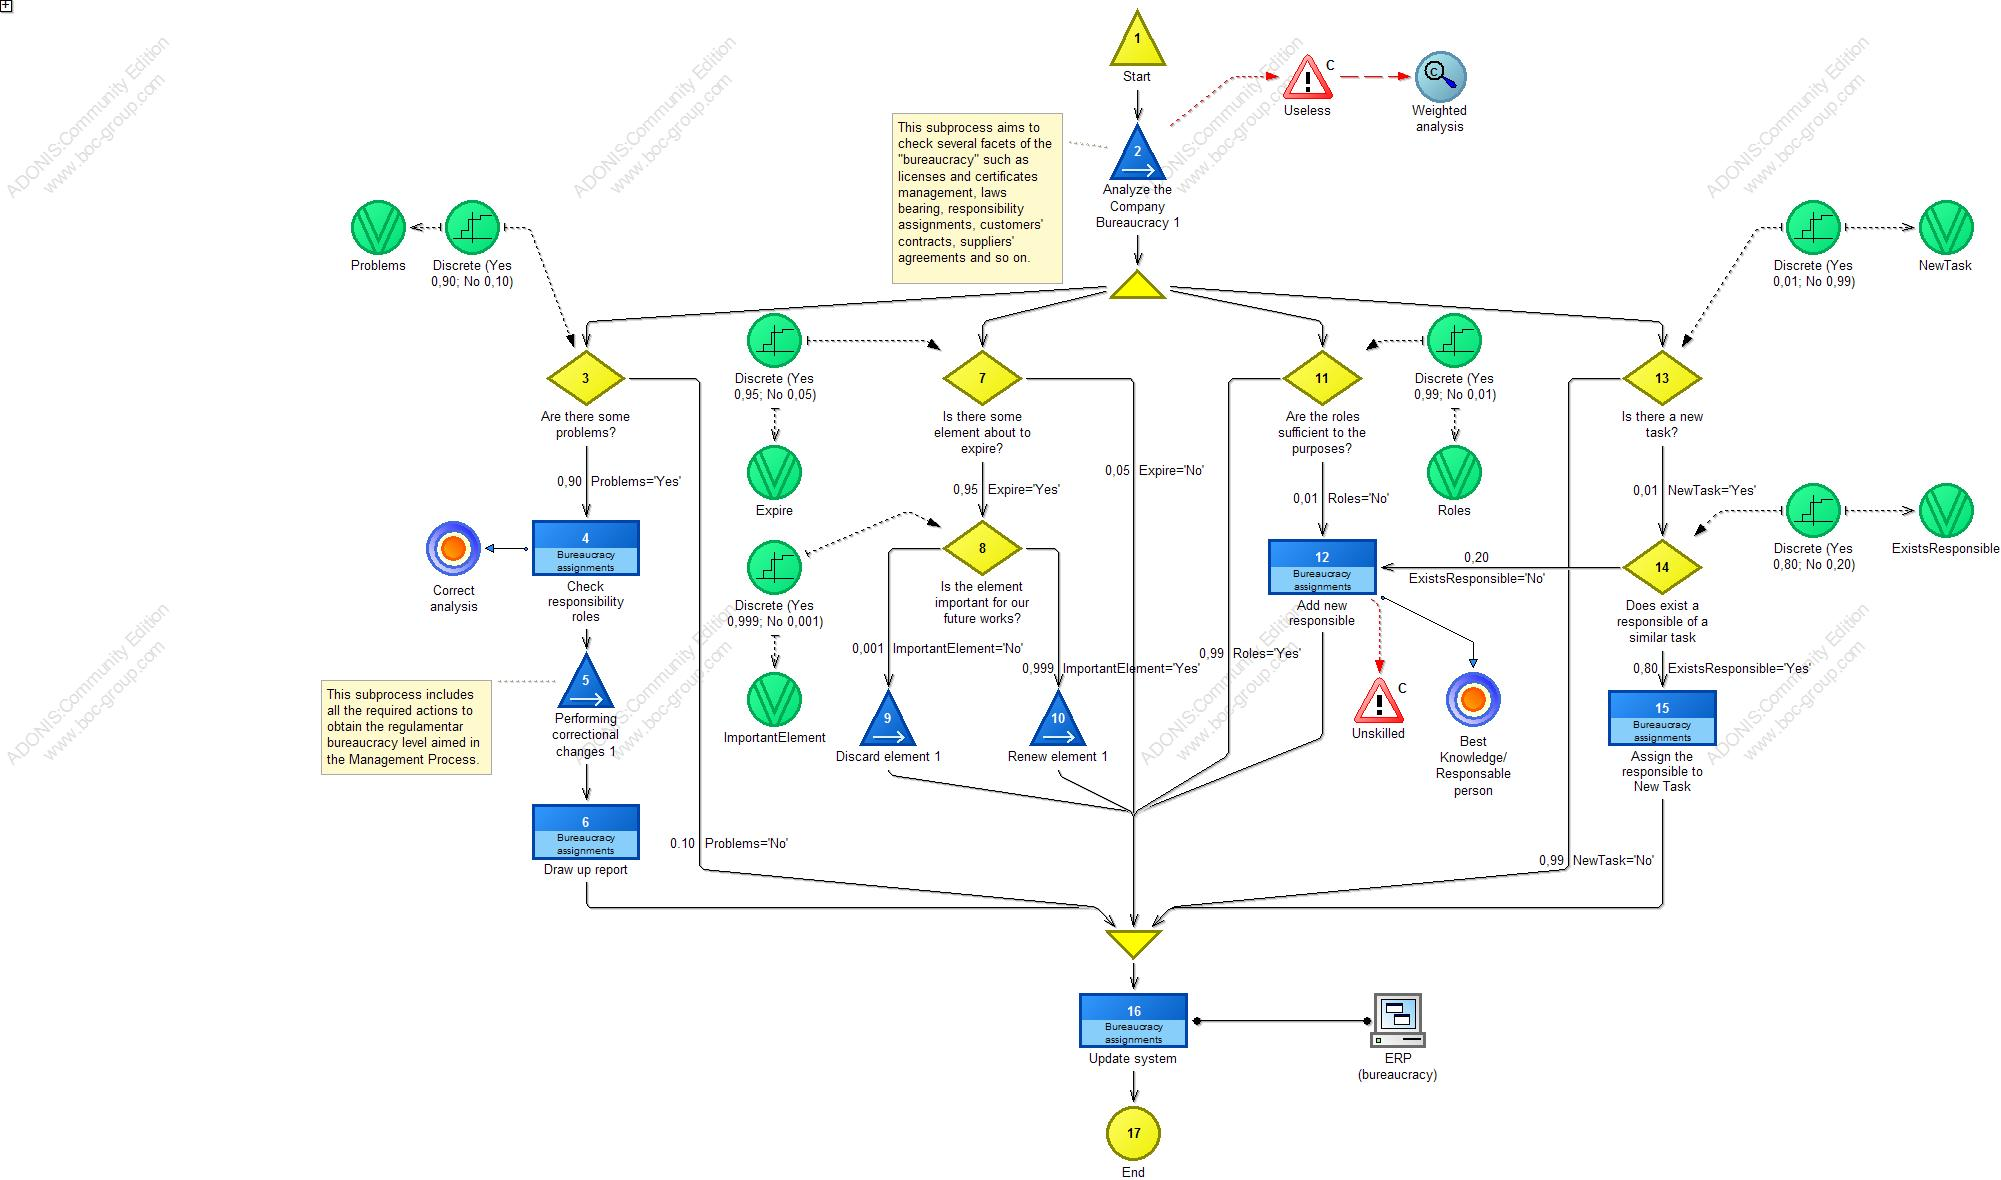
\includegraphics[scale=0.35, angle=90]{assign2/adonis/imgs/financial_sup.jpg}
\caption{AllSpark financial support.}
\label{2img:financial_sup}
\end{centering}
\end{figure}

\noindent
\emph{Path Analysis}\\
The path analysis shows fifteen paths which three of them really important. The following table illustrate their characteristics.\\

\begin{table}
\centering
\begin{tabular}{|l|l|l|l|l|}
Path&Probability&Execution time&Cycle time&Costs\\
\hline
1&0,6120&00:000:02:15:00&00:000:03:01:00&66,20\\
\hline
2&0,1650&00:000:02:55:00&00:000:03:01:00&116,20\\
\hline
3&0,1010&00:000:03:05:00&00:000:03:16:00&66,20
\end{tabular}
\end{table}

The favorite path is the first and it is presented as follows.\\

\begin{alltt}
Probability:   61,2000%
Execution time:  00:000:02:15:00
Waiting time:  00:000:00:28:00
Resting time:  00:000:00:18:00
Transport time:  00:000:00:10:00
Cycle time:  00:000:03:01:00
Costs:  66,200000

Financial support 0.2 (Business process model)
========================================
Process start: Start
Parallelity: Parallelity-37548
    *
    Activity: Loading financial data
    *
    Activity: Focusing the task
    Decision: Are the owned skills sufficients? --> OwnedKnowledge='Yes'

Merging: Merging-37551
Activity: Perform business activity
Activity: Update Company information
Parallelity: Parallelity-37615
    *
    Decision: Is the financial status of AllSpark right? --> FinancialStatusOk='Yes'
    *
    Decision: Company is working right? --> WorkingOk='Yes'
    Activity: Next trend
    *
    Decision: Is AllSpark ready for change? --> TimeChanging='No'
Merging: Merging-37618
Activity: Draw up report and notify results to CEO
End: End
\end{alltt}

\noindent
\emph{Capacity Analysis}\\
The capacity analysis of the process figures as expectations that the business consultant is the primary role in the task and basically the business process is a sequential step of his work.

\begin{landscape}
\centering
{\tiny
\begin{tabular}{|l|l|l|l|l|l|l|}
Business process&Activity&Performer&Number&Execution time&Cycle time&Costs\\
\hline
Financial support 0.2&&&&00:000:02:33:28&00:000:03:04:50&77,040900\\
\hline
&Loading financial data&&1,000000&00:000:00:07:00&&0,300000\\
\hline
&&Business consultant&1,000000&00:000:00:07:00&&0,300000\\
\hline
&Focusing the task&&1,034000&00:000:00:10:20&&0,051700\\
\hline
&&Analyst&1,034000&00:000:00:10:20&&0,051700\\
\hline
&Update Company information&&1,000000&00:000:00:03:00&&0,800000\\
\hline
&&Secretary&1,000000&00:000:00:03:00&&0,800000\\
\hline
&Draw up report and notify results to CEO&&1,000000&00:000:00:20:00&&0,050000\\
\hline
&&Business consultant&1,000000&00:000:00:20:00&&0,050000\\
\hline
&Gathering informations&&0,034000&00:000:00:01:01&&0,027200\\
\hline
&&Business consultant&0,034000&00:000:00:01:01&&0,027200\\
\hline
&Plan a suggetion strategy&&0,229000&00:000:00:09:10&&11,450000\\
\hline
&&Business consultant&0,229000&00:000:00:09:10&&11,450000\\
\hline
&Historical study&&0,022000&00:000:00:00:26&&0,022000\\
\hline
&&Secretary&0,022000&00:000:00:00:26&&0,022000\\
\hline
&Plan changing&&0,170000&00:000:00:08:30&&0,000000\\
\hline
&&Business consultant&0,170000&00:000:00:08:30&&0,000000\\
\hline
&Next trend&&0,978000&00:000:00:44:01&&29,340000\\
\hline
&&Business consultant&0,978000&00:000:00:44:01&&29,340000\\
\hline
&Perform business activity&&1,000000&00:000:00:50:00&&35,000000\\
\hline
&&Business consultant&1,000000&00:000:00:50:00&&35,000000\\
\hline
Total&&&&00:000:02:33:28&&77,040900
\end{tabular}
}
%\caption{Capacity analysis for Financial support.}
\end{landscape}
%

%

\subsection{Marketing Management}
This process provides support for the definition of the appropriate
remuneration for the service supplied.
The process takes into account the history of project development and the details defined in the contract, in order to check if they match or if some extra features have been during the development phase. The employees mainly involved are Business Consultant, Secretary and the CEO.

Image \ref{2img:billing} shows how this process is realized in practice, focusing on the resources used and the targets for each activity. The goal of this process is to provide a fair billing to the customer, balanced on the services actually delivered.\\

\begin{figure}[ht!]
\begin{centering}
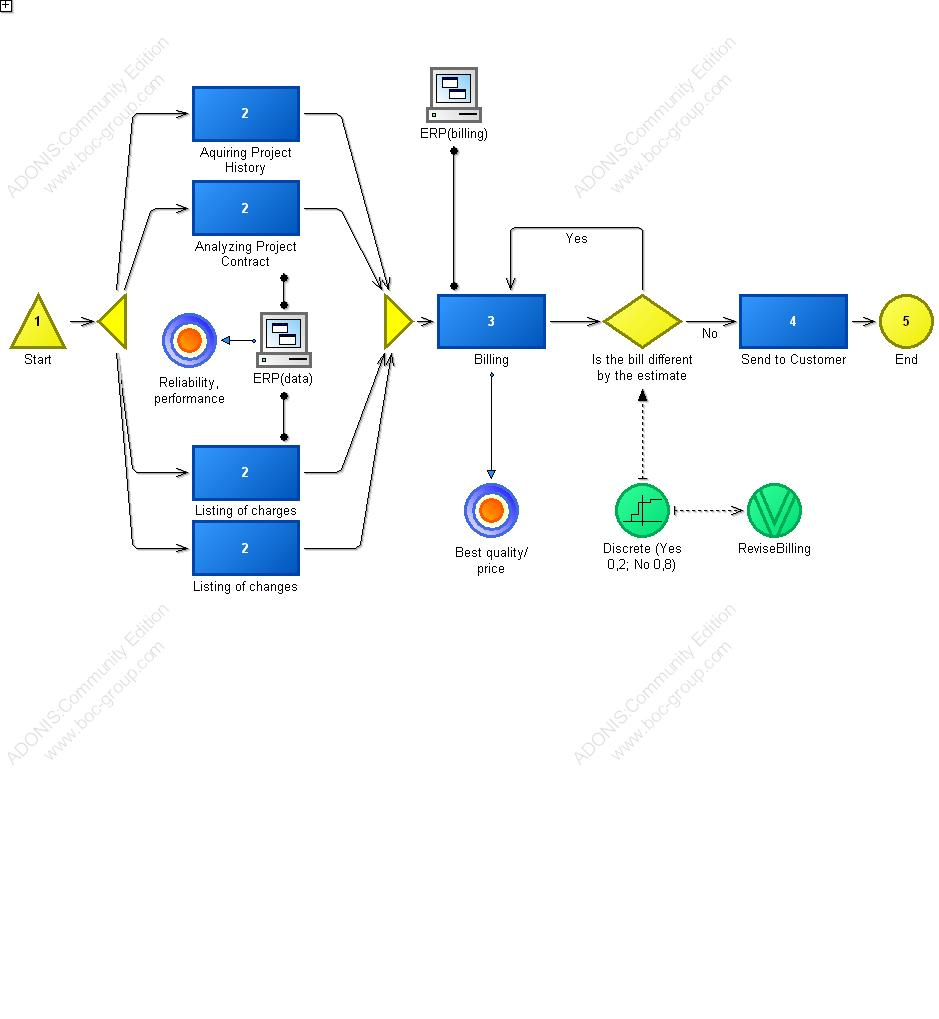
\includegraphics[scale=0.50, angle=90]{assign2/adonis/imgs/billing.jpg}
\caption{AllSpark billing process.}
\label{2img:billing}
\end{centering}
\end{figure}

\noindent
\emph{Path Analysis}\\
The analysis of possible paths results five correspondence, one with the 80,40\% of probability to be performed. For simulation's convention the number of these processes per month is configured on three element on average.

\begin{alltt}

\end{alltt}

\noindent
\emph{Capacity Analysis}\\
The capacity analysis of the process illustrates the specified timing and costs forseen for the single activities. Morevover it exlicities the Performer associated to each activity in order to check the responsibility for each step of the Business Process.

\begin{landscape}
\centering
{\tiny
\begin{tabular}{|l|l|l|l|l|l|l|}
Business process&Activity&Performer&Number&Execution time&Cycle time&Costs\\
\hline

\end{tabular}
}
%\caption{Capacity analysis for Marketing management.}
\end{landscape}
%

%

\subsection{Public Relation Management}
